%%%%%%%%%%%%%%%%%%%%%%%%%%%%%%%%%%%%%%%%%%%%%%%%%%%%%
% Author: [Francesco Giraudo]
% Date: 2025-03-17
% Description: [Exercise Set 1 - Computational Finance]
%%%%%%%%%%%%%%%%%%%%%%%%%%%%%%%%%%%%%%%%%%%%%%%%%%%%%

\documentclass{article}
\usepackage[english]{babel}
\usepackage{amsfonts}
\usepackage{amsmath} 
\usepackage{amssymb}
\usepackage{graphicx}
\usepackage{geometry}
\usepackage{mdframed}

\renewcommand{\thesubsection}{\thesection.\alph{subsection}} % Letter for subsections

% Set custom margins
\geometry{
  top=0.75in,
  bottom=0.75in,
  left=0.78in,
  right=0.78in
}

% Eliminate paragraph indentation
\setlength{\parindent}{0pt}

\title{Computational Finance - Exercise set 01}
\author{Francesco Giraudo \\ \small{Vrije Universiteit} \\ {\small\texttt{f.giraudo@student.vu.nl}}}
\date{24 March 2025}

\begin{document}

\maketitle

\section{Exercise 1}

\subsection{}

I want to show theoretically that
\begin{equation}
    \int_0^t W(s)ds = \int_0^t (t-s)dW(s)
\end{equation} \\

Considering the function $g(s,X(s)) = (t-s)X(s)$ where $X(s):=W(s)$ and applying Ito's lemma
\begin{equation*}
d\,g(s,X(s)) = \frac{\partial g}{\partial g} ds +
               \frac{\partial g}{\partial X(s)} dX(s)
            = X(t)\,dt + t\,dX(t)
\end{equation*}

Integrating both sides and substituting $g(s,X(s))=(t-s)X(s)$ and $X(s)=W(s)$ I obtain

\begin{align*}
    \int_0^t{d\left[(t-s)W(s)\right]} &=  -\int_0^t{W(s)\,ds} \;+ \int_0^t{(t-s)\,dW(s)} \\
    (t-s)W(t) \left|^t_0 \right. &= -\int_0^t{W(s)\,ds} \;+ \int_0^t{(t-s)\,dW(s)} \\
    (t-t)W(t) - (t-0)W(0) &= -\int_0^t{W(s)\,ds} \;+ \int_0^t{(t-s)\,dW(s)} \\ 
    -tW(0) &= -\int_0^t{W(s)\,ds} \;+ \int_0^t{(t-s)\,dW(s)}
\end{align*}

Since $W(t)$ is a Wiener process, by definition $W(0)=0$ w.p. $1$, so I can conclude that

\begin{align*}
    -\int_0^t{W(s)\,ds} \;&+ \int_0^t{(t-s)\,dW(s)} = 0 \\ 
    \int_0^t{W(s)\,ds} &= \int_0^t{(t-s)\,dW(s)} \qquad \qquad \square
\end{align*}

\subsection{}

This section presents the numerical validation of the theoretical equality $\int_0^t W(s)ds = \int_0^t (t-s)dW(s)$ with $t=5$.

The time interval $[0,5]$ was discretized into $n$ equal subintervals of length $\Delta t = \frac{5}{n}$ with time points $t_i = i\Delta t$ for $i = 0,1,2,...,n$. The left-hand side integral was approximated using a left-point Riemann sum: $\int_0^5 W(s)ds \approx \sum_{i=0}^{n-1} W(t_i) \Delta t$. The right-hand side stochastic integral was approximated using the Itô discretization: $\int_0^5 (5-s)dW(s) \approx \sum_{i=0}^{n-1} (5-t_i)[W(t_{i+1})-W(t_i)]$.

The numerical implementation calculated these approximations recursively:
\begin{align}
I1(t_{i+1}) &= I1(t_i) + W(t_i)\Delta t\\
I2(t_{i+1}) &= I2(t_i) + (5-t_i)[W(t_{i+1})-W(t_i)]
\end{align}

\begin{figure}[H]
\centering
% Insert first figure here
\includegraphics[width=0.8\textwidth]{brownian_paths_figure.png}
\caption{Sample path of Brownian motion and the two integral processes showing their equality}
\label{fig:paths}
\end{figure}

Figure \ref{fig:paths} displays one realization of a Brownian motion path along with both integral processes. Visual inspection confirms the integrals track each other closely throughout the time period, providing initial evidence of their equality.

For rigorous validation, 1,000 independent paths were simulated using step sizes ranging from $2^1$ to $2^{15}$. The absolute difference between terminal values was calculated: $\text{Error} = \left|\int_0^5 W(s)ds - \int_0^5 (5-s)dW(s)\right|$.

\begin{figure}[H]
\centering
% Insert second figure here
\includegraphics[width=0.8\textwidth]{convergence_figure.png}
\caption{Mean absolute error convergence with 95\% confidence intervals}
\label{fig:convergence}
\end{figure}

Figure \ref{fig:convergence} shows the mean absolute error decreasing as the number of steps increases, following approximately an $O(1/n)$ convergence rate. The 95\% confidence intervals (calculated as $\text{Mean Error} \pm 1.96 \times \frac{\text{Standard Deviation}}{\sqrt{1000}}$) narrow with increasing step count, indicating reduced variability in the approximation error.

The numerical experiment strongly validates the theoretical equality. The mean absolute error approaches zero as discretization becomes finer, reaching approximately $1.5 \times 10^{-4}$ at $2^{15}$ steps. This convergence behavior provides compelling evidence for the theoretical result established in part (a). The small remaining error is attributable to the inherent limitations of numerical discretization and would continue to decrease with finer discretization.


\newpage

\section{Exercise 2}

\subsection{}

I want to find the dynamics of $Y_1(t) := \mu S^2(t)$ where $S(t)$ is a geometric Brownian motion defined as follows

\begin{equation}
    dS(t) =  \mu S(t) + \sigma S(t)dW(t) \label{eq:GBMdef2}
\end{equation}

with $\mu$ and $\sigma$ are constant parameters and $W(t)$ the Wiener process. \\ 

Let consider the function $g(t,S(t)) = \mu S^2(t) = Y_1(t)$, applying Ito's lemma I obtain

\begin{align}
    dg(t,S(t)) &= \frac{\partial g}{\partial t} dt +
                    \frac{\partial g}{\partial S(t)} dS(t) +
                    \frac{1}{2} \frac{\partial^2g}{\partial S^2(t)} (dS(t))^2\label{eq:itoformula}\\
    dY_1(t) &= \, 0 + 2\mu S(t)\,dS(t) + \frac{1}{2}\,2\mu\,(dS(t))^2 \;=\; 2\mu S(t) dS(t) + \mu (dS(t))^2 \label{eq:line2}
\end{align}

Now, let's analyze $(dS(t))^2$. Using the definition of GBM in (\ref{eq:GBMdef2}) and Ito's multiplication table rule for simplifying the terms, it follows that:

\begin{align}
    (dS(t))^2 &= [\mu S(t)dt + \sigma S(t)dW(t)]^2 \notag\\
              &= (\mu S(t))^2 dtdt + 2\sigma S(t) dW(t) dt + (\sigma S(t))^2 dW(t)dW(t) \notag \\
              &= 0 + 0 + \sigma^2 S^2(t) dt \label{eq:dS2t} 
\end{align}

Substituting (\ref{eq:dS2t}) into equation (\ref{eq:line2}) and given that $Y_1(t)=\mu S^2(t)$, I find
\begin{align*}
d Y_1(t) &= (2\mu S(t))\,(\mu S(t) + \sigma S(t)dW(t))+ \sigma^2 \mu S^2(t) dt \\
         &= (2\mu+\sigma^2) \mu S^2(t)dt + 2\mu S^2(t) dW(t) \\
         &= (2\mu+\sigma^2) Y_1(t)\,dt + 2Y_1(t) \,dW(t)
\end{align*}

Thus, I can conclude $Y_1(t)$ is a GBM with parameters $\tilde{\mu}= (2\mu+\sigma^2)$ and $\tilde{\sigma} = 2$.

\subsection{}

Using Ito's formula with $g(t,W(t)) := e^{W(t)}$, I have

\begin{align}
dg(t,W(t)) &= \frac{\partial g}{\partial t} dt +
              \frac{\partial g}{\partial W(t)} dW(t) +
              \frac{1}{2} \frac{\partial^2g}{\partial W^2(t)} (dW(t))^2 \label{eq:itoformula2}
\end{align}

Calculating the derivatives and using the definition of $Y_2(t)$, it follows that

\begin{align*}
dY_2(t) &= 0\,dt + e^{W(t)}\,dW(t) + \frac{1}{2}e^{W(t)}\,(dW(t))^2 \\
        &= \frac{1}{2}e^{W(t)}\,dt +  e^{W(t)}\,dW(t) \\
        &= \frac{1}{2}Y_2(t)\,dt + Y_2(t)\,dW(t)
\end{align*}

The stochastic process $Y_2(t)$ is a GBM with parameters $\mu=\frac{1}{2}$ and $\sigma=1$, so it is not a martingale because the drift term $\mu$ is not zero.

\newpage

\section{Exercise 3}

The standardization procedure ensures that the random samples from a normal distribution maintain a mean of 0 and a variance of 1, aligning with the theoretical assumptions of the Black-Scholes model.

The Black-Scholes model assumes that stock prices follow a geometric Brownian motion, requiring normally distributed random variables with specific statistical properties. In the simulation, stock price paths are generated according to
\begin{equation}
    S_{t+\Delta t} = S_t \exp\left((r - \frac{1}{2}\sigma^2)\Delta t + \sigma\sqrt{\Delta t}Z\right),
\end{equation}
where $Z \sim N(0,1)$ represents standard normal random variables. In practice, computer-generated random numbers may not perfectly maintain these statistical properties, particularly with smaller sample sizes.

The analytical price of a European call option is computed using the Black-Scholes formula:
\begin{equation}
    C = S_0 \Phi(d_1) - K e^{-rT} \Phi(d_2),
\end{equation}
where
\begin{equation}
    d_1 = \frac{\ln(S_0 / K) + (r + \frac{1}{2} \sigma^2)T}{\sigma \sqrt{T}}, \quad d_2 = d_1 - \sigma \sqrt{T}.
\end{equation}
Here, $\Phi(\cdot)$ represents the cumulative distribution function of the standard normal distribution.

A Monte Carlo simulation is implemented to price a European call option using the following parameters:

\begin{center}
    \begin{tabular}{l c c}
        \toprule
        Parameter & Symbol & Value \\
        \midrule
        Initial Stock Price & $S_0$ & 100.0 \\
        Strike Price & $K$ & 95.0 \\
        Risk-free Rate & $r$ & 0.03 \\
        Volatility & $\sigma$ & 0.10 \\
        Time to Maturity & $T$ & 1.0 \\
        \bottomrule
    \end{tabular}
\end{center}

The analytical solution using the Black-Scholes formula yields a price of $8.934954$. Two versions of the Monte Carlo simulation were compared: one using standardized random samples to ensure a mean of 0 and standard deviation of 1, and another using raw random samples directly. The convergence is tested by varying the number of simulation paths from 2 to 10000. \\

\vspace{0.25cm}

\begin{figure}[h!]
\centering
\begin{minipage}{0.5\textwidth}
    \centering
    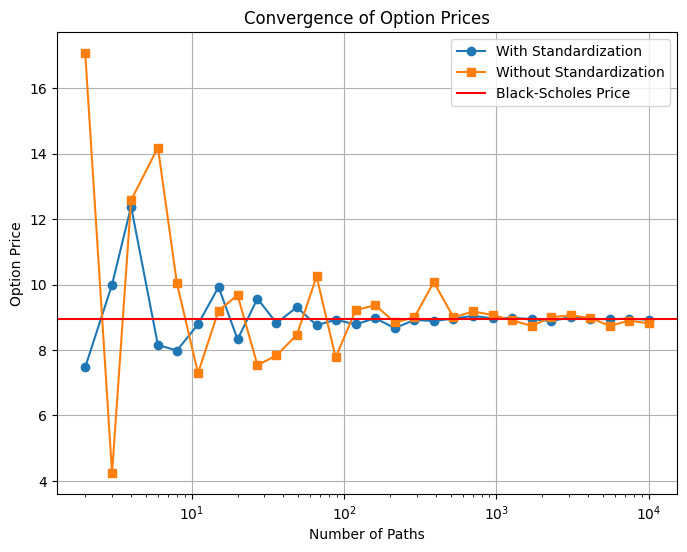
\includegraphics[width=0.95\textwidth]{Exercise_set_01/img/ConvergenceStdVsNon.png}\\
    \caption{Convergence of option price estimates with and without standardization}
    \label{fig:StdVsNonConv}
\end{minipage}%
\begin{minipage}{0.5\textwidth}
    \centering
    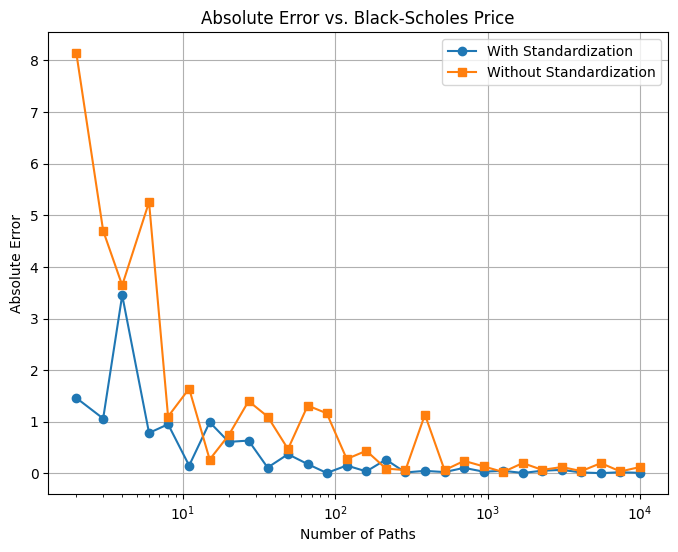
\includegraphics[width=0.95\textwidth]{Exercise_set_01/img/ConvergenceAbsValue.png}\\
    \caption{Absolute error in option price estimates with and without standardization}
    \label{fig:StdVsNonAbs}
\end{minipage}
\end{figure}

\vspace{0.5cm}

Figures \ref{fig:StdVsNonConv} and \ref{fig:StdVsNonAbs} illustrate the effect of standardization on the convergence and accuracy of Monte Carlo option price estimates. The standardized method exhibits greater stability, especially when the number of simulation paths is small, leading to a smoother and more consistent convergence toward the analytical Black-Scholes price.\\
In contrast, the non-standardized approach shows significant fluctuations at lower path counts, with price estimates displaying considerable variability. The absolute error plot further highlights the advantage of standardization, as it consistently results in lower errors across different path counts. The non-standardized approach, on the other hand, produces substantially larger errors, particularly when the number of paths is below 100, demonstrating its inefficiency in scenarios with limited simulations. \\

In addition to this, stability analysis is performed using 1000 different random seeds with a fixed path count of 100.\\

\begin{figure}[h!]
\centering
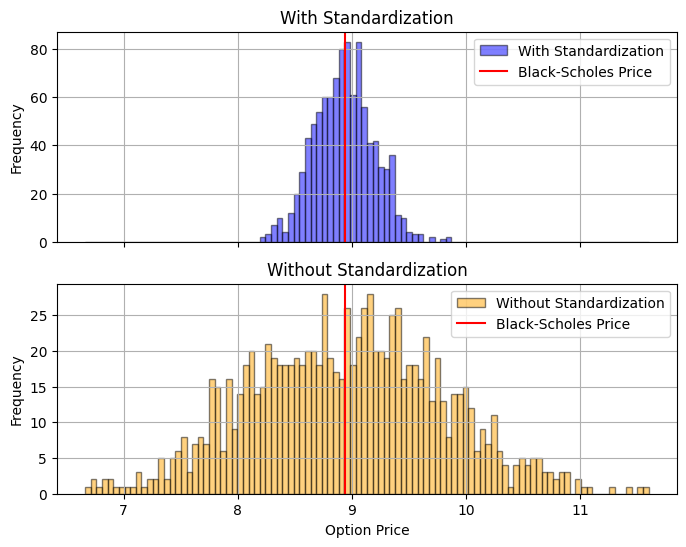
\includegraphics[width=0.5\textwidth]{Exercise_set_01/img/DistStdVsNon.png} \
\caption{Standardization vs without standardization option price estimation}
\label{fig:distStdVsNon}
\end{figure}

\begin{center}
\begin{tabular}{l c c c}
\toprule
Method & Mean Price & Standard Deviation & Mean Absolute Error \\
\midrule
With Standardization & 8.933259 & 0.260974 & 0.208185 \\
Without Standardization & 8.951233 & 0.845786 & 0.686860 \\
Black-Scholes (Analytical) & 8.934954 & - & - \\
\bottomrule
\end{tabular}
\end{center}

The distribution of option prices from simulations with 1000 different random seeds is presented in Figure (\ref{fig:distStdVsNon}). The standardized method produces a tighter, more normally distributed set of prices centered closely around the analytical Black-Scholes price. The non-standardized method yields a wider, more irregular distribution with greater variance. Furthermore, one observes that with standardization, the mean price of 8.933259 closely approximates the analytical Black-Scholes price of 8.934954, with a standard deviation of merely 0.260974. In contrast, the non-standardized approach yields a mean price of 8.951233 with a substantially higher standard deviation of 0.845786. The mean absolute error confirms this superior performance, with the standardized method achieving 0.208185 compared to 0.686860 for the non-standardized approach. \\

The standardization process effectively functions as a variance reduction technique, producing more consistent results with fewer simulation paths. This effect is evident in the significantly lower standard deviation of the standardized method compared to the non-standardized approach. By enforcing the theoretical properties of normal random variables with mean 0 and variance 1, one ensures that the simulation adheres more closely to the theoretical model's assumptions, thereby enhancing the accuracy and reliability of the option pricing estimates. The improved statistical precision consequently leads to faster convergence, requiring fewer paths to achieve comparable accuracy to the analytical solution. \\

To sum up, standardizing random samples in Monte Carlo simulations for option pricing under the Black-Scholes model provides significant benefits in terms of accuracy, efficiency, and reliability. The standardized approach converges faster to the analytical solution, exhibits lower variability across different random seeds, and produces consistently lower errors compared to the non-standardized method.

\newpage

\section{Exercise 4}

\subsection{Analytical value of $\text{Var}(X(t))$}

For a Wiener process $W(t)$, consider the process:
\begin{equation*}
X(t) = W(t) - \frac{t}{T}W(T-t), \quad \text{for } 0 \leq t \leq T.
\end{equation*}

For the definition of the Wiener process, it is known that $\mathbb{E}[W(t)]=0$ and $\text{Var}(W(t))=t$. \\

Firstly, the expectation of $X(t)$ is computed
\begin{align*}
\mathbb{E}[X(t)] &= \mathbb{E}\left[W(t) - \frac{t}{T}W(T-t)\right] \\
&= \mathbb{E}[W(t)] - \frac{t}{T}\mathbb{E}[W(T-t)] \\
&= 0 - \frac{t}{T} \cdot 0 = 0
\end{align*}

Next, the variance of $X(t)$ is derived as follows
\begin{equation*}
\text{Var}(X(t)) = \mathbb{E}[X^2(t)] - (\mathbb{E}[X(t)])^2 = \mathbb{E}[X^2(t)]
\end{equation*}

Expanding $X^2(t)$, I find that
\begin{align*}
X^2(t) &= \left(W(t) - \frac{t}{T}W(T-t)\right)^2 \\
&= W^2(t) - 2\frac{t}{T}W(t)W(T-t) + \frac{t^2}{T^2}W^2(T-t)
\end{align*}

Taking the expectation,
\begin{align}
\mathbb{E}[X^2(t)] &= \mathbb{E}[W^2(t)] - 2\frac{t}{T}\mathbb{E}[W(t)W(T-t)] +
                      \frac{t^2}{T^2}\mathbb{E}[W^2(T-t)] \label{eq:expX2}
\end{align}

Using the properties of the Wiener process stated before, I can simply find that
\begin{align}
\mathbb{E}[W^2(t)] = t \qquad \text{and} \qquad \mathbb{E}[W^2(T-t)] = T-t \label{eq:expvarW}
\end{align}

To compute $\mathbb{E}[W(t)W(T-t)]$, the property of independent increments of the Wiener process is used. \\

Assume $s \leq t$. Then, it is possible to decompose $W(t)$ as $W(t) = W(s) + (W(t) - W(s))$.
Since $W(t) - W(s)$ is independent of $W(s)$ and has mean zero,
\begin{align*}
\mathbb{E}[W(s)W(t)] &= \mathbb{E}[W(s)(W(s) + (W(t) - W(s)))] \\
&= \mathbb{E}[W(s)^2] + \mathbb{E}[W(s)(W(t) - W(s))] \\
&= s + 0 = s
\end{align*}

Thus, for $s \leq t$, we have $\mathbb{E}[W(s)W(t)] = s$. By symmetry, for $t \leq s$, we have $\mathbb{E}[W(s)W(t)] = t$. Therefore, in general $\mathbb{E}[W(s)W(t)] = \min(s, t).$
Applying this result to $\mathbb{E}[W(t)W(T-t)]$, substituting $s = t$ and $t = T - t$, it follows that
\begin{equation*}
    \mathbb{E}[W(t)W(T-t)] = \min(t, T - t)
\end{equation*}

This gives the piecewise expression:
\begin{align}
\mathbb{E}[W(t)W(T-t)] = 
\begin{cases}
t, & \text{if } t \leq \frac{T}{2}, \\
T - t, & \text{if } t > \frac{T}{2}. \label{eq:covW}
\end{cases}
\end{align}

Now that all the values are finally known, it is possible to substitute the results (\ref{eq:expvarW}) and (\ref{eq:covW}) into the expression (\ref{eq:expX2}), obtaining
\begin{align*}
\mathbb{E}[X^2(t)] &= t - 2\frac{t}{T}\min(t, T-t) + \frac{t^2}{T^2}(T-t).
\end{align*}

Thus, the variance of $X(t)$ is given by the expression
\begin{equation*}
\text{Var}(X(t)) = t - 2\frac{t}{T}\min(t, T-t) + \frac{t^2}{T^2}(T-t).
\end{equation*}

In particular for $T = 10$, this simplifies to
\begin{equation}
\text{Var}(X(t)) = 
\begin{cases}
t - \frac{t^2}{5} + \frac{t^2(10-t)}{100}, & \text{if } t \leq 5, \\
t - \frac{t(10-t)}{5} + \frac{t^2(10-t)}{100}, & \text{if } t > 5. \label{eq:var_t}
\end{cases}
\end{equation}

\subsection{Numerical Simulation}

 For numerical confirmation, I simulated 100000 paths of $X(t)$ and estimated the variance in 1000 time steps over the time interval $[0,T]$ with $T = 10$. The Wiener process $W(t)$ was approximated by generating random increments, which were then accumulated to produce a discretized representation of the continuous process. This discretized process was used to compute the values of $X(t)$ at each time step.

To estimate the variance of $X(t)$, the sample variance was calculated across all simulated paths at each time step. Then, this numerical estimate was compared with the analytical expression (\ref{eq:var_t}) derived before.

\begin{figure}[h!]
\centering
\begin{minipage}{0.5\textwidth}
    \centering
    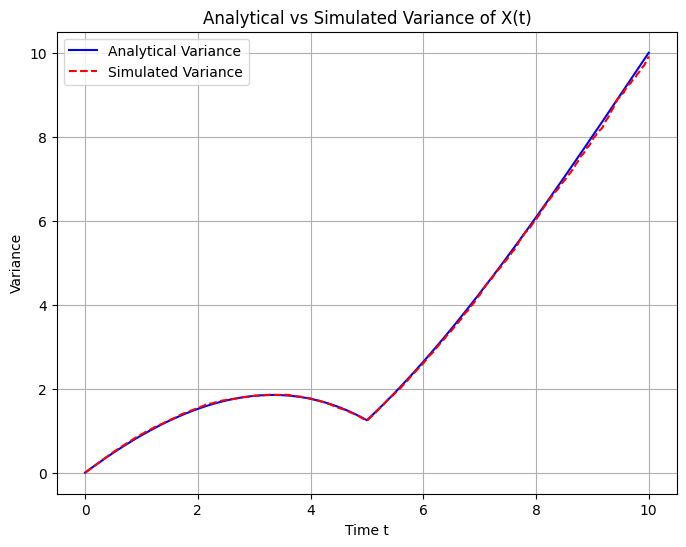
\includegraphics[width=1\textwidth]{Exercise_set_01/img/AnalyticalVsSimulated.png}
    \caption{Analytical vs Simulated Variance of \(X(t)\)}
    \label{fig:var}
\end{minipage}%
\begin{minipage}{0.5\textwidth}
    \centering
    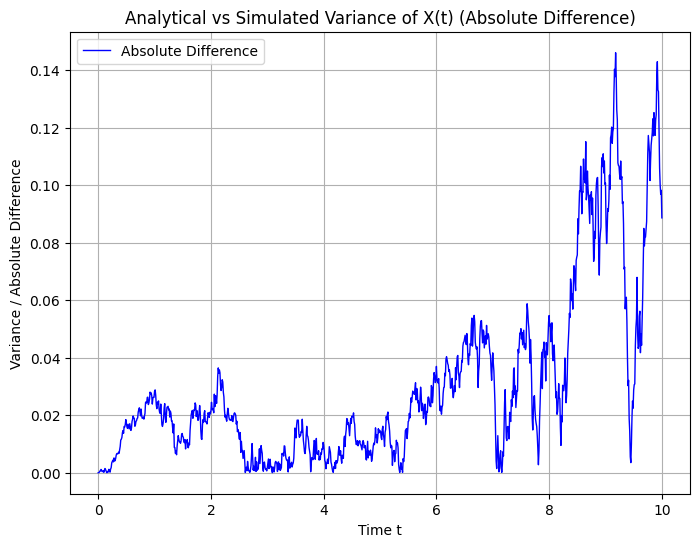
\includegraphics[width=1\textwidth]{Exercise_set_01/img/AnalyticalVsSimulated_abs.png}
    \caption{Absolute Difference Between Analytical and Simulated Variance of \(X(t)\)}
    \label{fig:diff}
\end{minipage}
\end{figure}

The results show agreement between the simulated and analytical variances, as shown in Figure \ref{fig:var}. However, in Figure \ref{fig:diff} it is possible to see accuracy differences between $t\leq5$ and $t\leq10$. In fact, for $t \leq 5$, the difference remains consistently low and stable, indicating a high level of precision in this region. Instead, for $t \geq 5$, the error begins to increase slightly, with a more noticeable rise as $t$ approaches $T=10$. In conclusion, it seems that the accuracy is sensitive to $t$.
\newpage

\end{document}
